% !TEX root = ../../../main/aws_chabauty.tex
\newpage
\section{Jennifer Balakrishnan: Computational tools for quadratic Chabauty}
\subsection{Lecture 1}

\begin{ques}
Does there exist a pair of rational right triangles and a rational isoceles triangle that have the same area and the same perimeter?
\end{ques}

	\begin{figure}[!ht]
	\centering
	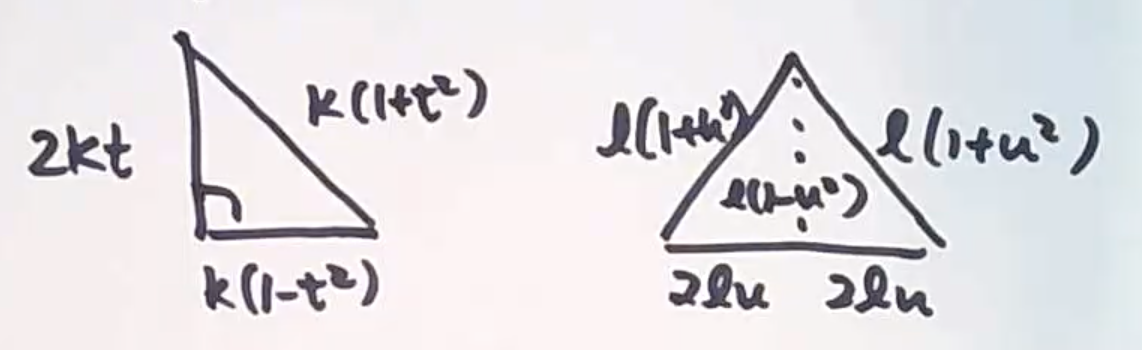
\includegraphics[width=0.6\textwidth]{../images/im4.png}
	\end{figure}

We rescale $l=1$, suppose $k,t,u \in \Q$, $0<?,u<1$, $k>0$

Equate areas and perimeters:

% Formulas

After some algebra, we see there exists $x \in \Q$, $1<x<2$ such that $2xk^2+(-3x^2-2x^2+6x-4)k+x^5= 0$. The discriminant of polynomial in $k$ must be a rational square:
	\[
	\begin{aligned}
	y^2&= (-3x^2-2x^2+6x-4)^2-4(2x)x^5 \\
	&=x^6+12x^5-32x^4+52x^2-48x+16
	\end{aligned}
	\]
This is a genus 2 curve, and we'd like to determine $X(\Q)$. The Jacobian $J$ of $X$ has rank $\rank J(\Q)=1$. Also, Chabauty-Coleman bound gives $\#X(\Q) \leq 10$. We can find $\{\infty^\pm, (0,\pm 4), (1,\pm 1), (2, \pm 8), (12/11,\pm 868/11^3) \} \subseteq X(\Q)$. We've found no rational points!


The answer to the discriminant question:


\begin{thm}[Hirakawa-Matsumura, 2018]
Yes, there are exactly one pair of such triangles.
\end{thm}



% Coleman's Effective Chabauty
\subsubsection{Coleman's Effective Chabauty}

Let $X/\Q$ be a `nice' curve with genus $g \geq 2$. Suppose that $\rank J(\Q)< g$. If $p>2g$ is good, then $\#X(\Q) \leq \#X(\F_p) + 2g - 2$. This bound comes from bounding the number of zeros of a $p$-adic (Coleman) integral.


Coleman gave a theory of $p$-adic line integration in the 1980s. 


\begin{thm}[Coleman]
Let $X/\Q_p$ be a nice curve with good reduction at $p$. The $p$-adic itnegral $\int_P^Q \omega \in \ov{\Q}_p$, defined for $P,Q \in X(\ov{\Q}_p)$ and $\omega \in H^0(X,\Omega^1)$ satisfies the following:

\begin{enumerate}[(i)]
\item the integral is $\ov{\Q}_p$ linear in $\omega$
\item if $P,Q$ reduce to the same point $\ov{P} \in X(\ov{\F}_p)$, then we call the integral a `tiny' integral.
\item We have
	\[
	\int_P^Q \omega + \int_{P'}^{Q'} \omega= \int_P^Q \omega + \int_{P'}^Q \omega
	\]
then we can define $\int_D^\omega$ for $D= \sum_{j=1}^n ((Q_j)-(P+j)) \in DN_K^0(\ov{\Q}_p)$ as $\int_P \omega= \sum_{j=1}^n \int_{P_j}^{Q_j} \omega$.
\item if $D$ is principal, then $\int_D \omega= 0$.
\item Integral compatibility with $\Gal(\ov{\Q}_p/\Q_p)$-action.
\item Fix $P_0 \in X(\ov{\Q}_p)$. If $0 \neq \omega \in H^0(?,\Omega^1)$, then the set of points $P \in X(\ov{\Q}_p)$ reduces to a fixed point on $X(\F_p)$ such that $\int_{P_0}^{P_1} \omega= 0$ is finite. 
\end{enumerate}
\end{thm}


This is the Coleman integral. Cont Given hypotheses of previous theorem, let $b \in X(\Q_p)$, $i: X \hra J$ given by $P \mapsto [P-b]$. There is a map $J(\Q_p) \times H^0(X_{\Q_p},\Omega^1) \to \Q_p$ given by $(Q,\omega) \mapsto \langle Q,\omega \rangle$ that's additive in $Q$, $\Q_p$-linear in $\omega$, and given by $\langle [D],\omega \rangle= \int_D \omega$ for $D \in \div_X^0$.


For $P \in X(\Q_p)$, we have the Abel-Jacobi morphism $Aj_b$ that takes $P$ to 
	\[
	\langle i(P), \omega \rangle= \int_b^P \omega =: AJ_b(P)
	\]
The Chabauty-Coleman method uses a certain subspace of the space of regular 1-forms. Now assume $b \in X(\Q)$, use it to embed $X \hra J$.


\begin{dfn}
Let $A= \{ \omega \in H^0(X,\Omega^1) \text{ for all } P \in J(\Q), \langle P,\omega \rangle=0 \}$ be the subspace of annihilating differentials.  
\end{dfn}


We have
	\[
	\begin{tikzcd}
	X(\Q) \arrow{d} \arrow{r} & X(\Q_p) \arrow{d} \arrow{dr}{AJ_b} \\
	J(\Q) \arrow{r} & J(\Q_p) \arrow{r}{\log} &  H^0(J_{\Q_p},\Omega^1) \simeq H^0(X_{\Q_p}, \Omega^1)
	\end{tikzcd}
	\]
By ``computing rational points via Chabauty-Coleman: compute the finite set of $p$-adic points
	\[
	X(\Q_p)_1:= \{ z \in X(\Q_p) \colon \int_b^z \omega= 0 \text{ for all } \omega \in A \}
	\]
By construction, $X(\Q) \subset X(\Q_p)$. How do we compute annihilating differ?


\begin{ex}
Let $X: y^2= x^5-2x^3+x=1$ (LMFBD: 971.4 971.1) Some facts about $X$:
\begin{enumerate}[(i)]
\item $X(\Q)_{\text{known}}= \{ \infty, (0,\pm1/2), (-1,\pm1/2), (1,\pm 1/2)\}$
\item $J$ is simple, $J(\Q) \simeq \Z$, $[(-1,-1/2)-(0,1/2)] \in J(\Q)$ has infinite order.
\item $X$ is good at $p=3$, $\#X(\F_3)=7$. Stoll's refinement of Chabauty-Coleman for $p= 3$:
	\[
	\#X(\Q) \leq \#X(\F_p) + 2 r + \dfrac{2r}{p-2}= 11
	\]
\end{enumerate}
So need to do more work to determine $X(\Q)$ here. We will construct a 3-adic annihilating differential $\eta$. Basts of $H^0(X_{\Q_p},\Omega^1)$ is $\left\{ \omega_i = \dfrac{x^i \;dx}{2y} \right\}_{i=0,1}$. So $\eta$ is a $\Q_3$-linear combination of $\omega_0, \omega$. We will compute the values of $\alpha;= \int_{(a,b)}^{1-\gamma_0} \omega_0$ and $\beta:= \int_{(0,\gamma_0)}^{1-\gamma_0} \omega$ to compute $\eta$. SageMath can compute $\alpha, \beta$
	\[
	\begin{aligned}
	\alpha&= 3+3^2+3^4+\cdots \\
	\beta&= 2 + 2\cdot 3 + 2 \cdot 3^2 + \cdots
	\end{aligned}
	\]
We take $\eta= \beta \omega_0 - \alpha \omega_1$ and run Chabauty-Coleman. 
\end{ex}


Where do these numbers come from?



% Explicit Coleman Integration
\subsubsection{Explicit Coleman Integration}

Using the action of Frobenius on $p$-adic cohomology. (Sage for hyperelliptic curves or Magma for plane curves.) Let $X^\an$ denote the rigid analytic space over $\Q_p$ associated to $X/\Qp$. A wide open subspace of $X^\an$, the complement in $X^\an$ of the union of a finite collection of disjoint closed disks of radius $<1$. Now for some more properties of the Coleman integral:

\begin{thm}[Coleman]
Let $\eta, \xi$ be 1-forms on a wide open $V$ of $X^\an$, $P,Q, R \in V(\ov{\Qp})$, let $a,b \in \ov{\Qp}$. Then we have 
\begin{enumerate}[(i)]
\item linearity in integrand:
	\[
	\int_P^Q a\eta + b \xi= a \int_P^Q \eta + b \int_P^Q \xi
	\]
\item additivity in endpoints
	\[
	\int_P^R \eta + \int_R^Q \eta= \int_P^Q \eta
	\]
\item change of variables under rigid analytic maps (Frobenius)
\item Fundamental Theorem of Calculus
	\[
	\int_P^Q df= f(P) - f(Q)
	\]
\item Galois compatability
\end{enumerate}
\end{thm}


We first integrate $\int_P^Q \omega$ for $\omega$ 1-form of the second kind, $P, Q \in V(\Qp)$. Suppose $X$ is a hyperelliptic curve. Sketch of explicit Coleman integration (B-Bradshaw-Kedlaya).


\begin{enumerate}[1.]
\item take a lift of $p$-power Frobenius
\item compute a basis $\{ \omega_i \}$ of 1-forms of the second kind
\item compute $\phi^* \omega_i$ via Kedlaya's zeta function algorithm and use properties of Coleman integral to relate
	\[
	\int_P^Q \phi^*\omega_i \text{ to } \int_P^Q \omega_i
	\]
as well as other easier terms.
\item solve for $\int_P^Q \omega_i$ using lth. algorithm.
\end{enumerate}
 

We sketch Kedlaya's algorithm. Let $X$ be the curve $y^2= p(x)$. We work in an affine $Y \subset X$ given by defining Weierstrass points. Take $\phi$ to be $x \mapsto x^p$ and $y \mapsto y^p \sum_{j=0}^\infty \binom{1/2}{1} \left( \dfrac{p(x^p - p(x)^p}{y^{2p}} \right)^j$. Then we compute the action of $\phi$ on
	\[
	\begin{aligned}
	\phi^*\left( \dfrac{x^i \;dx}{y} \right)&= \dfrac{x^{pi} \;d(x^p)}{\phi(y)} \\
	&= \dfrac{x^{pi} p x^{p-1} \;dx}{\phi(y)} \\
	&= p x^{pi + p - 1} y^{-p} \sum_{j=0}^\infty \binom{1/2}{1} \left( \dfrac{p(x^p - p(x)^p}{y^{2p}} \right)^j
	\end{aligned}
	\]
and reduce pole order of each resulting differential using relations in $H^1$. Denote the basis by $\{\omega_i\}_{i=0,\ldots,2g-1}$. Then Kedlaya's algorithm gives
	\[
	\phi^* \omega_i= dh_o + \sum_{j=0}^{2g-1} \mu_{ji} \omega_j
	\]
If we can compute $h_i$ and $M$, then
	\[
	\begin{pmatrix}
	\vdots \\
	\int_P^Q \omega_i \\
	\vdots
	\end{pmatrix}=
	(M^t - I)^{-1} 
	\begin{pmatrix}
	\vdots \\
	h_i(P) - h_i(Q) - \int_P^{\pi(P)} \omega_i - \int_{\phi(Q)}^Q \omega_i \\
	\vdots
	\end{pmatrix}
	\] % *


Finishing the 3-adic integrals on $y^2= x^5 - 2x^3 + x + 1/4$, we constructed $\eta= \beta \omega_0 - \alpha \omega_1$, where $\alpha,\beta$ are computed using (*). We want to compute $X(\Q_3)$. Compute power series expansions of
	\[
	\left\{ \int_{(0,1/2)}^{P_t} \eta \right\}
	\]
where $P_t$ ranges over all residue disks:
	\[
	\int_{(0,1/2)}^{P_t} \eta= \underbrace{\int_{(0,1/2)}^{P_0} \eta}_{\text{Gives 3-adic}} + \underbrace{\int_{P_0}^{P_t} \eta}_{\text{Coleman 3-adic series}}
	\]
Lucky fact: For each residue disk, there exists $P_0 \in X(\Q)$, the 3-adic number is 0. Compute the tiny integral in each residue disk, we find each just has a simple zero at known rational point. This proves that $\#X(\Q)= 7$. 








 